\chapter{Zusammenfassung und Ausblick}
\label{ch:ausblick}

Im Rahmen dieser Arbeit werden zunächst die theoretische Grundlagen für das Verständnis der physikalischen und mathematischen Inhalte sowie
verschiedene Isolator-Modelle, insbesondere das Hubbard- und das Heisenberg-Modell, und Herleitungen für den IFE in Metallen und Isolatoren präsentiert.
Durch ein mikroskopisches Festkörpersystem, bestehend aus vier Gitterplätzen und jeweils zwei Spin-Niveaus, wird ein Mott-Hubbard-Isolator modelliert
und untersucht. Der Übergang vom Mott-Hubbard-Isolator in den Mott-Heisenberg-Isolator bei einer besonders starken Coulomb-Wechselwirkung zwischen den Elektronen
$U \gg J$ wird anhand des betrachteten Systems festgestellt und damit die Erwartung bestätigt.
Im nächsten Schritt wird für die Untersuchung des IFE in dem modellierten Isolator ein hochfrequent rotierendes E-Feld eingeschaltet.
Es wird gezeigt, dass kein Strom und somit auch keine Magnetisierung mittels des IFE in dem Festkörpersystem angeregt wird. Der  resultierende Widerspruch
zu der vorgestellten Herleitung für den IFE in Isolatoren lässt vermuten, dass das System für die Nachstellung des IFE in Mott-Isolatoren zu klein ist.
Diese Annahme ist unter anderem darauf gestützt, dass für einen Hubbard-Parameter $U=0$ ebenfalls im Langzeitmittel kein Stromfluss beobachtet wird,
obwohl das Festkörpersystem in diesem Fall keinen Isolator repräsentiert.
Darüberhinaus wird die Vermutung aufgestellt, dass die Teilchen-Loch-Symmetrie des Systems für die Beobachtung, dass kein Strom angeregt wird, verantwortlich ist.
Diese lässt sich jedoch nicht bestätigen, da bei Brechung der Teilchen-Loch-Symmetrie durch das Hinzufügen einer Übernächst-Nachbar-Tight-Binding-Wechselwirkung
weiterhin kein Stromfluss erzeugt wird.
Anhand der aufgestellten Annahmen ist es naheliegend, den IFE in einem vergrößerten Festkörpersystem, wie beispielsweise
in Abbildung \ref{fig:gitterausblick} gezeigt, zu untersuchen. Dabei ist zu beachten, dass mit jedem ergänzten Gitterplatz
die Hilbertraumdimension rapide ansteigt und somit die numerische Auswertung erschwert wird.

\begin{figure}
  \centering
  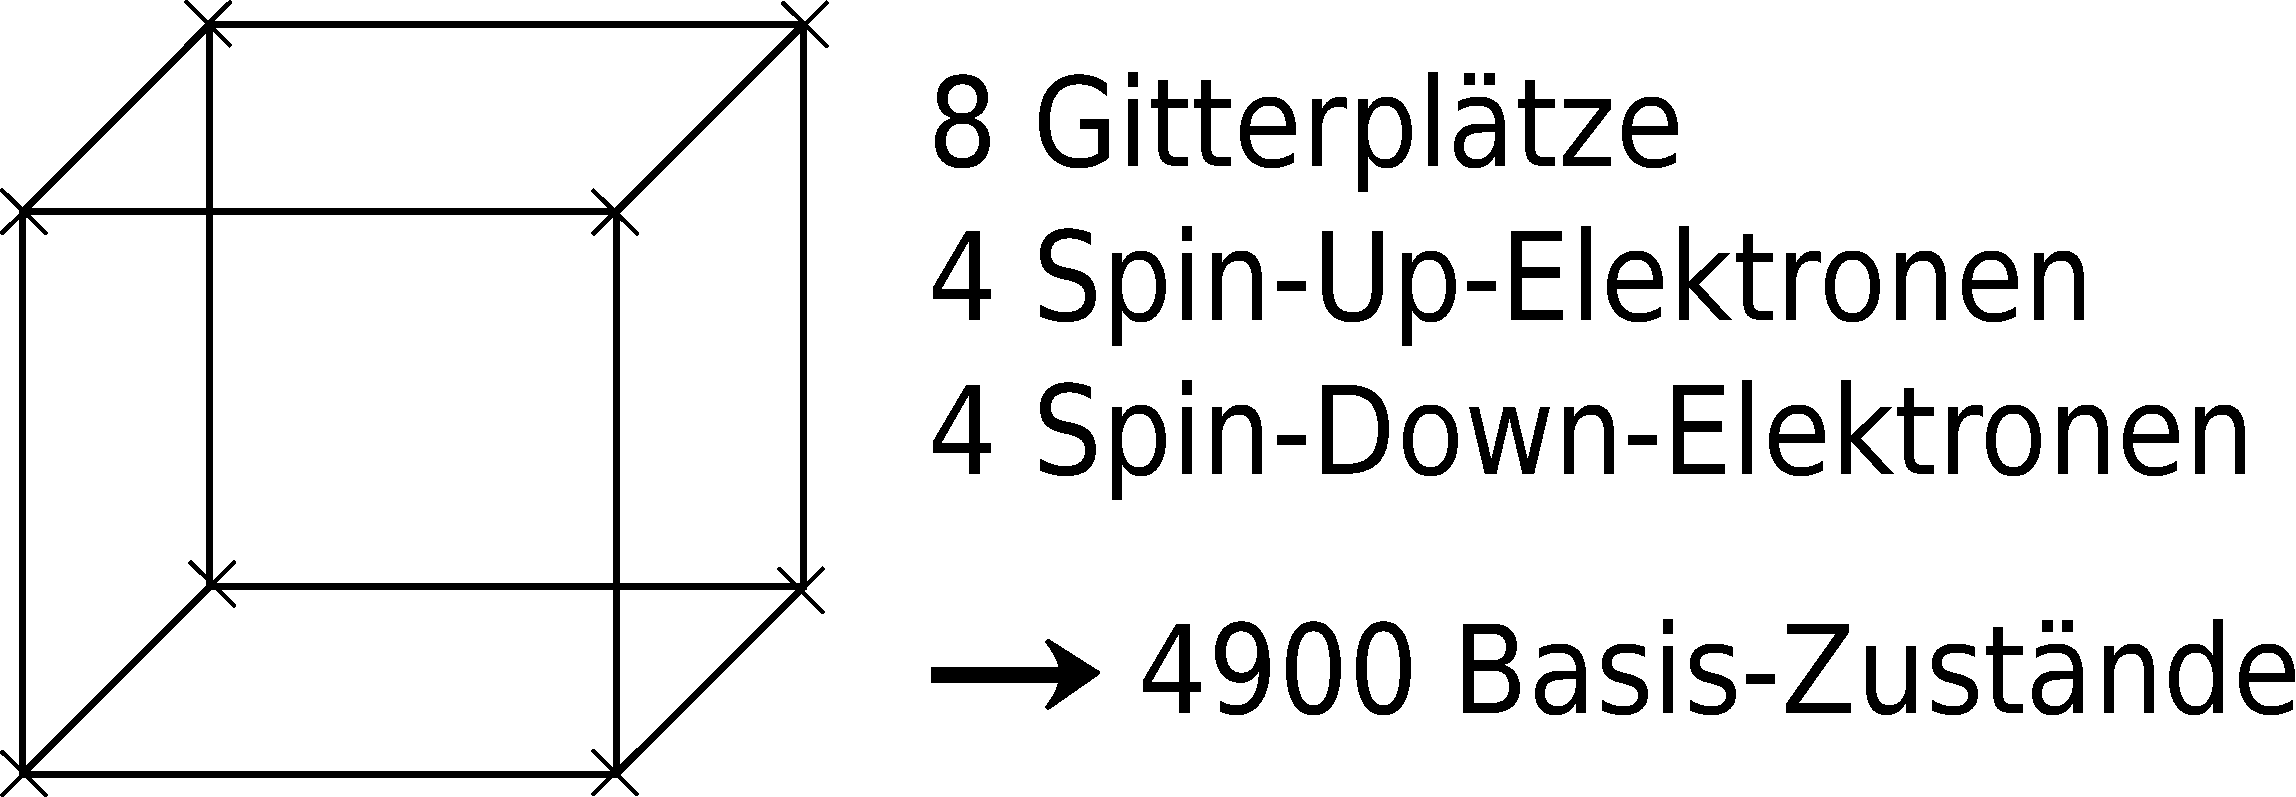
\includegraphics[height=2cm]{Graphiken/gitterausblick.pdf}
  \caption{Eine Möglichkeit zur Erweiterung des Gittersystems.}
  \label{fig:gitterausblick}
\end{figure}

Des Weiteren bleibt die Frage offen, ob durch die in Gleichung \eqref{eqn:isomag} aufgezeigte Formel für den IFE in Isolatoren
die Realität beschrieben wird. Es besteht daher sowohl Interesse an einer Herleitung des IFE, in der quantenmechanische
Effekte berücksichtigt werden, als auch an einer experimentellen Untersuchung des IFE in einem Mott-Isolator.
